% Figure 2 — Types of users (boxed tree, like the reference)
\documentclass[border=12pt]{standalone}
\usepackage{tikz}
\usetikzlibrary{arrows.meta}
\begin{document}
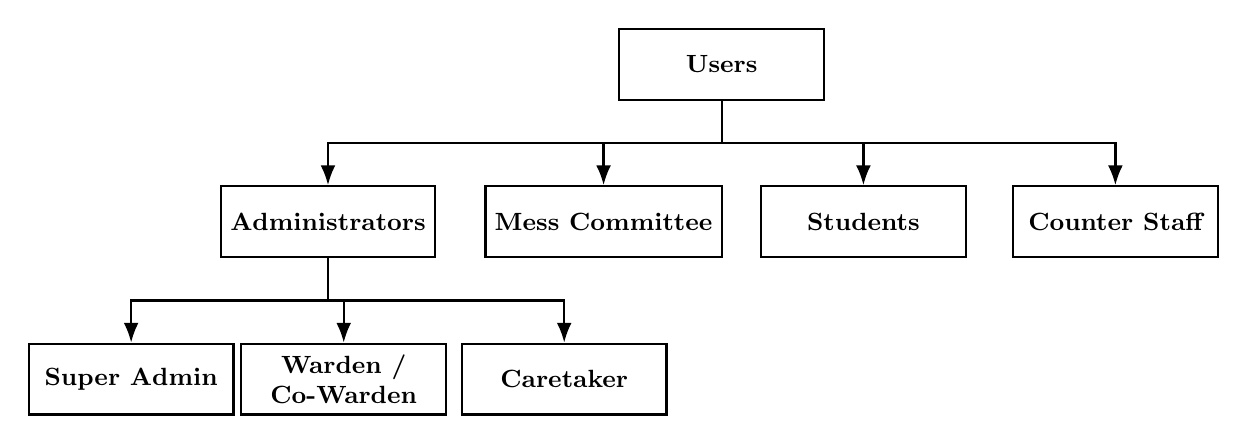
\begin{tikzpicture}[
    box/.style={rectangle, draw=black, thick, minimum width=2.6cm,
                minimum height=0.9cm, align=center, font=\bfseries\small},
    line/.style={-{Latex[length=2.5mm]}, thick},
  ]

  \node[box] (users) at (0, 6) {Users};

  \node[box] (admins)  at (-5, 4) {Administrators};
  \node[box] (committee) at (-1.5, 4) {Mess Committee};
  \node[box] (students) at (1.8, 4) {Students};
  \node[box] (staff)   at (5, 4) {Counter Staff};

  \node[box] (super)  at (-7.5, 2) {Super Admin};
  \node[box] (warden) at (-4.8, 2) {Warden /\\Co-Warden};
  \node[box] (care)   at (-2, 2) {Caretaker};

  % trunk down from Users
  \draw[line] (users) -- (0,5) -| (admins);
  \draw[line] (users) -- (0,5) -| (committee);
  \draw[line] (users) -- (0,5) -| (students);
  \draw[line] (users) -- (0,5) -| (staff);

  % admin children
  \draw[line] (admins) -- (-5,3) -| (super);
  \draw[line] (admins) -- (-5,3) -| (warden);
  \draw[line] (admins) -- (-5,3) -| (care);

\end{tikzpicture}
\end{document}
